\section{Diskussion}
\label{sec:Diskussion}
Die Abweichungen der errechneten Werte zu den Literaturwerten ist nicht sehr aussagekräftig, da das Material der Probekörper nur vermutet wurde.
Außerdem lässt sich für Messing nur ein Bereich finden, in dem sich das Elastizitätsmodul befindet, kein konkreter Wert.
Dadurch kann keine prozentuale Abweichung vom Literaturwert angegeben werden.\\

Abweichungen können auf Ungenauigkeit der Messuhren und Ablesefehler zurückgeführt werden.
Die Gewichte wurden während der Messung nicht verändert und waren nicht groß genug, sodass die Auslenkung oft kleiner als $\SI{3}{\milli\metre}$ waren.
Dann kann dort die Kleinwinkelnäherung nicht greifen.
Der Unterschied zwischen $0 \leq x \leq \frac{L}{2}$ und $\frac{L}{2}\leq x\leq L$ bei der beidseitigen Einspannung ist eventuell damit zu erklären, 
dass die Enden unterschiedlich fest eingespannt wurden. 
Der große Fehler von $E_2$ ist ein Indiz dafür, dass die Messung in diesem Bereich nicht genau war.

\section{Anhang}
\begin{figure}
    \centering
    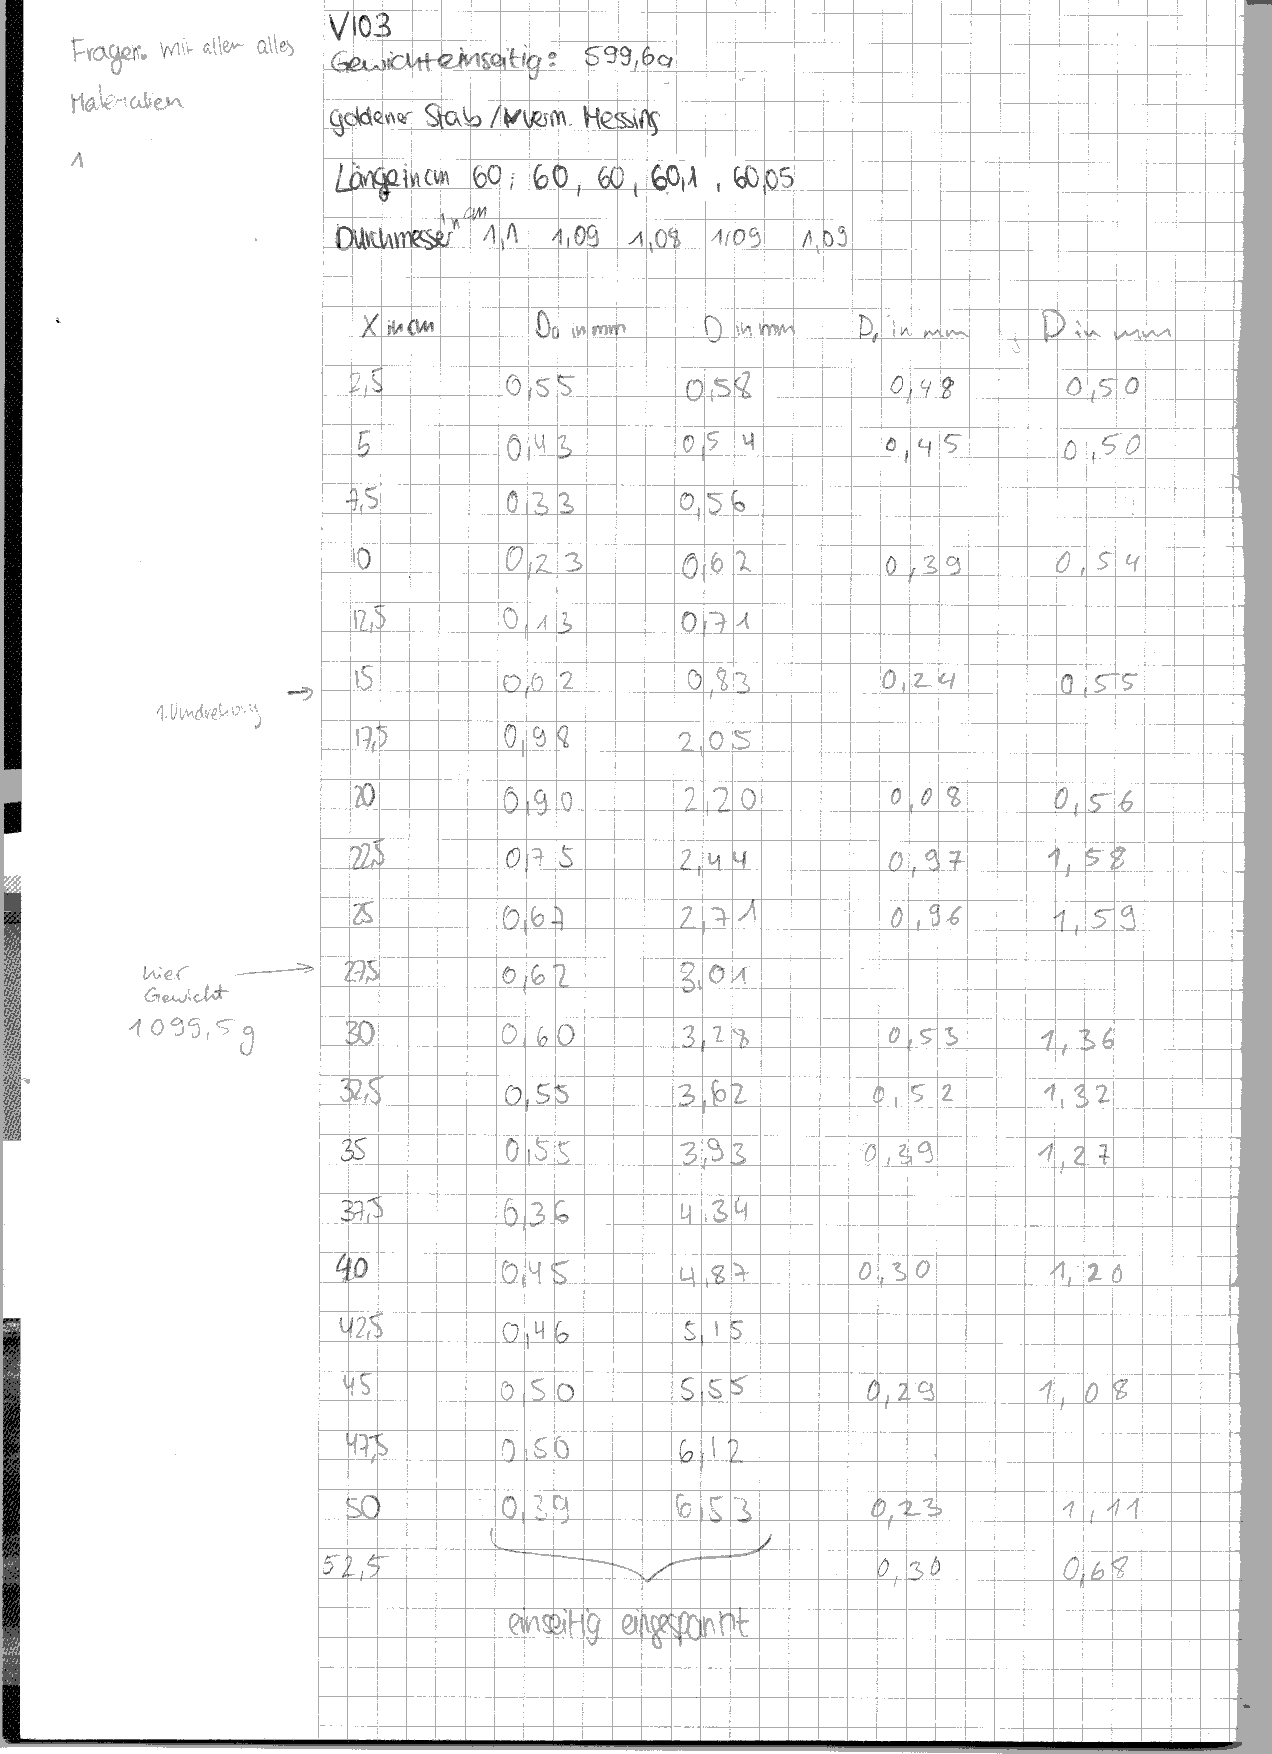
\includegraphics[width=\textwidth]{103_1.pdf}
\end{figure}
\begin{figure}
    \centering
    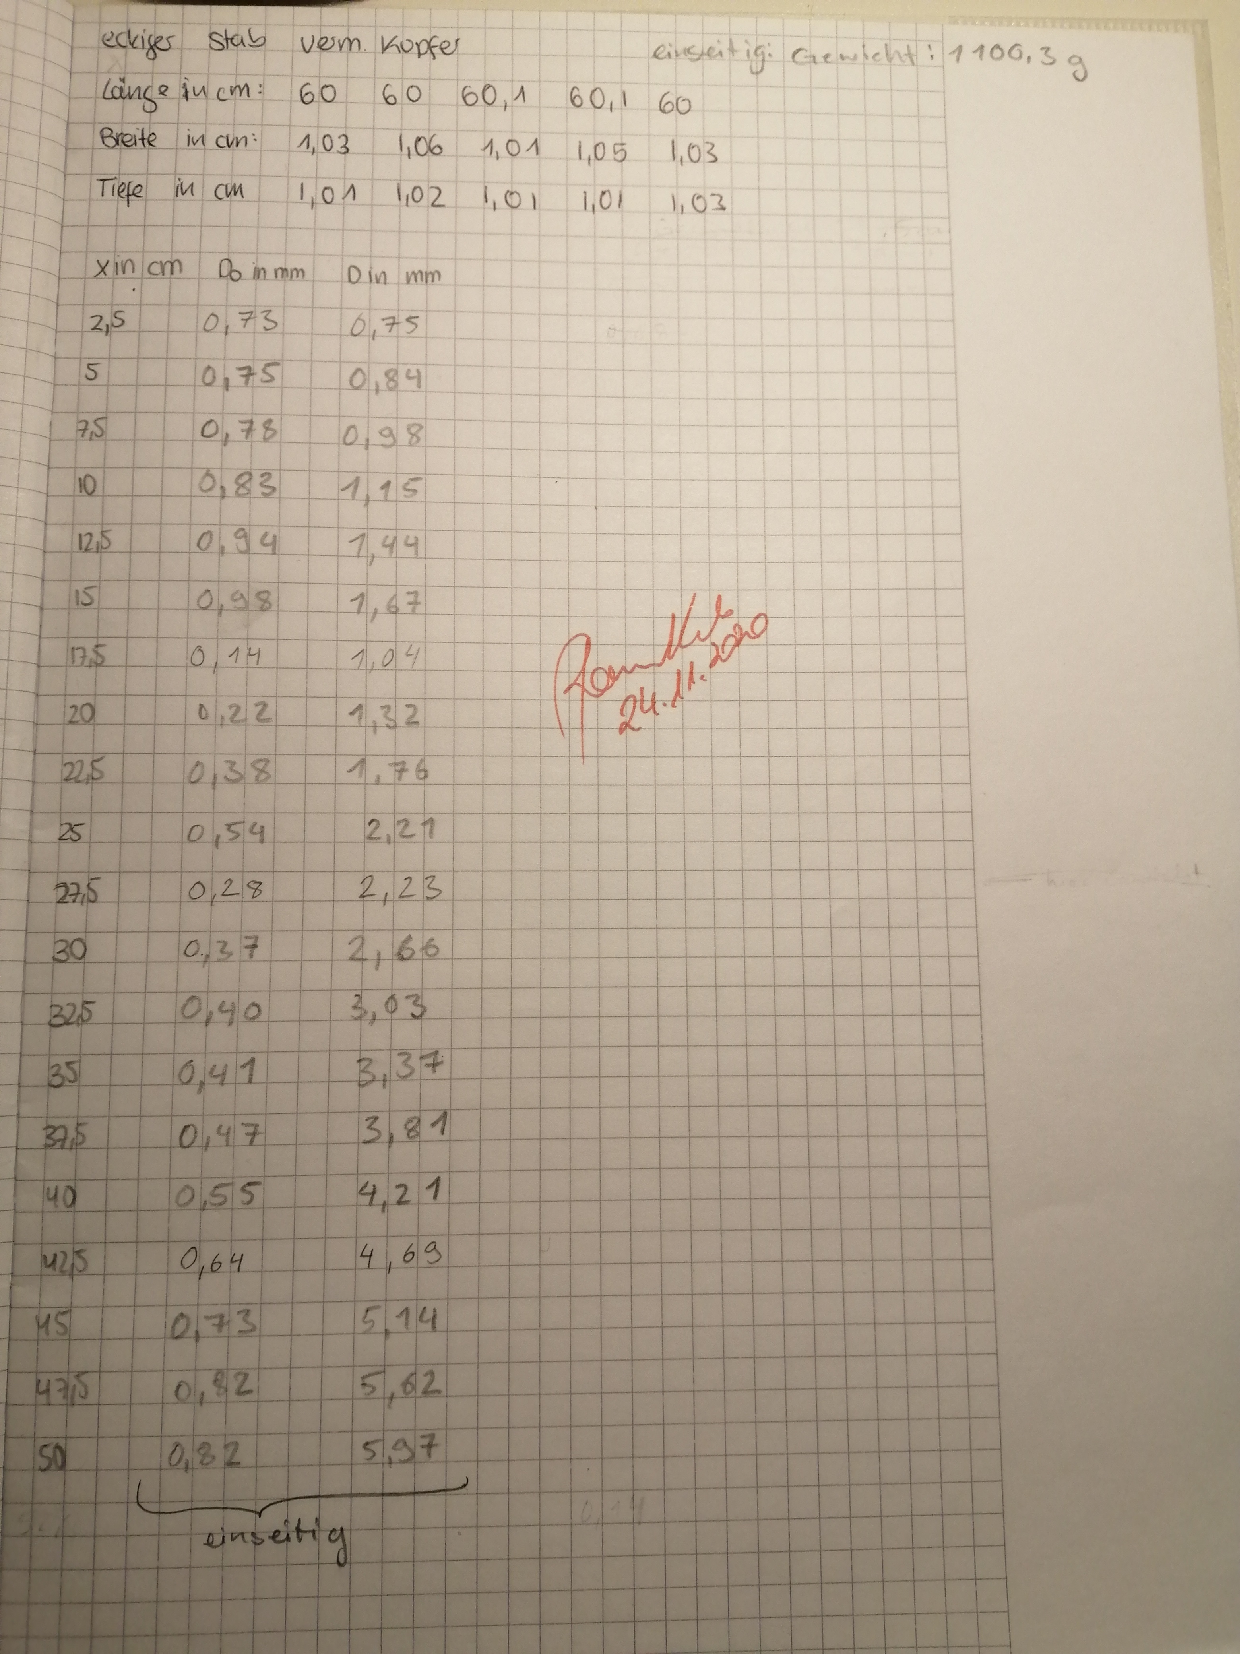
\includegraphics[width=\textwidth]{103_2-1.pdf}
\end{figure}
